%
% This is an example file and is hereby explicitly put in the
% public domain.
%
\documentclass[ppgc,diss,english]{iiufrgs}
% Para usar o modelo, deve-se informar o programa e o tipo de documento.
% Programas :
%   * cic       -- Graduação em Ciência da Computação
%   * ecp       -- Graduação em Ciência da Computação
%   * ppgc      -- Programa de Pós Graduação em Computação
%   * pgmigro   -- Programa de Pós Graduação em Microeletrônica
%
% Tipos de Documento:
%   * tc                -- Trabalhos de Conclusão (apenas cic e ecp)
%   * diss ou mestrado  -- Dissertações de Mestrado (ppgc e pgmicro)
%   * tese ou doutorado -- Teses de Doutorado (ppgc e pgmicro)
%   * ti                -- Trabalho Individual (ppgc e pgmicro)
%
% Outras Opções:
%   * english    -- para textos em inglês
%   * openright  -- Força início de capítulos em páginas ímpares (padrão da
%                   biblioteca)
%   * oneside    -- Desliga frente-e-verso
%   * nominatalocal -- Lê os dados da nominata do arquivo nominatalocal.def


% Use unicode
\usepackage[utf8]{inputenc}   % pacote para acentuação

% Necessário para incluir figuras
\usepackage{graphicx}           % pacote para importar figuras
\usepackage{tikz}

\usepackage{times}              % pacote para usar fonte Adobe Times
% \usepackage{palatino}
% \usepackage{mathptmx}          % p/ usar fonte Adobe Times nas fórmulas

\usepackage[alf,abnt-emphasize=bf]{abntex2cite}	% pacote para usar citações abnt

\usepackage{nicefrac}       % compact symbols for 1/2, etc.
\usepackage{amsfonts}       % blackboard math symbols
\usepackage{xspace}
\usepackage{amsmath}
\usepackage{amsthm}
\usepackage{amssymb}

\providecommand{\multiset}[1]{\ensuremath{\{\!\!\{#1\}\!\!\}}}
\providecommand{\sas}{\ensuremath{\text{SAS}^{+}}\xspace}
\providecommand{\strips}{STRIPS\xspace}
\providecommand{\astar}{\ensuremath{\text{A}^{*}}\xspace}
\providecommand{\gbfs}{\ensuremath{\text{GBFS}}\xspace}
\providecommand{\wida}{\ensuremath{\text{W-IDA}^{*}}\xspace}
\providecommand{\ida}{\ensuremath{\text{IDA}^{*}}\xspace}
\providecommand{\hvalue}[1]{\ensuremath{h^{#1}}\xspace}
\providecommand{\hstarp}[1]{\ensuremath{h^*({#1})}\xspace}
\providecommand{\hff}{\hvalue{\text{FF}}}
\providecommand{\hgc}{\hvalue{\text{GC}}}
\providecommand{\hstar}{\hvalue{*}}
\providecommand{\hlmc}{\hvalue{\text{lm-c}}}
\providecommand{\hmax}{\hvalue{\text{max}}}
\providecommand{\hadd}{\hvalue{\text{add}}}
\providecommand{\h}{$h$\xspace}
\providecommand{\hnn}{$\hat h$\xspace}
\providecommand{\hnrsl}{$\hat h^{\text{N-RSL}}$\xspace}
\providecommand{\hboot}{$\hat h^{\text{Boot}}$\xspace}
\providecommand{\hgc}{\hvalue{\text{gc}}}
\providecommand{\hhgn}{\hvalue{\text{HGN}}}
\providecommand{\unit}{/1\xspace}
\providecommand{\sui}{\text{SUI}\xspace}
\providecommand{\sai}{\text{SAI}\xspace}
\providecommand{\rw}{{RW}\xspace}
\providecommand{\bfs}{{BFS}\xspace}
\providecommand{\dfs}{{DFS}\xspace}
\providecommand{\bfsrw}{\text{FSM}\xspace}
\providecommand{\nn}{{NN}\xspace}
\providecommand{\fssp}{{FS}\xspace}
\providecommand{\bssp}{{BS}\xspace}
\providecommand{\hnnrs}{$\hat h{^{20\%}_\text{\meanfx}}$\xspace}
\providecommand{\hnnrsfifty}{$\hat h{^{50\%}_\text{\meanfx}}$\xspace}
\providecommand{\hffexp}{$h^{FF}_{exp}$}
\providecommand{\hgcexp}{$h^{GC}_{exp}$}
\providecommand{\hnnbase}{$\hat h_{0}$\xspace}
\providecommand{\hnnbfs}{$\hat h_{\text{bfs}}$\xspace}
\providecommand{\hnndfs}{$\hat h_{\text{dfs}}$\xspace}
\providecommand{\hnnrw}{$\hat h_{\text{rw}}$\xspace}
\providecommand{\hnnbfsrw}{$\hat h_\text{fsm}$\xspace}
\providecommand{\hnnbfsrwl}[1]{\ensuremath{\hat h_{#1}}\xspace}
\providecommand{\hnnnomutex}{\ensuremath{\hat h^{'}}\xspace}
\providecommand{\hnnnomutexl}[1]{\ensuremath{\hat h^{'}_{#1}}\xspace}
\providecommand{\hnnrsp}[1]{\ensuremath{\hat h_\text{fsm}/^{#1\%}_{\text{RS}}}\xspace}
\providecommand{\hnnrslp}[2]{\ensuremath{\hat h_\text{fsm}^{#1}/^{#2\%}_{\text{RS}}}\xspace}
\providecommand{\define}[1]{#1}
\providecommand{\facts}{\ensuremath{L_F}\xspace}
\providecommand{\meanfx}{\ensuremath{L_{\overline{F}}}\xspace}
\providecommand{\default}{\ensuremath{L_{200}}\xspace}
\providecommand{\distfarthest}{\ensuremath{d^*}\xspace}
\providecommand{\po}[1]{\ensuremath{\hat po^{#1}}\xspace}
\providecommand{\pot}[1]{\ensuremath{po^{#1}}\xspace}
\providecommand{\pog}{\po{\text{G}}}
\providecommand{\pofsm}{\po{\text{B}}}
\providecommand{\pogthresh}{\po{\text{G-thresh}}}
\providecommand{\pogmax}{\po{\text{G-max}}}
\providecommand{\popfa}{\po{\text{PFA}}}
\providecommand{\popfo}{\po{\text{PFO}}}
\providecommand{\postar}{\po{*}}
\providecommand{\postartable}{\pot{*}}
\providecommand{\pogstar}{\po{\text{G}^*}}
\providecommand{\pogstarthresh}{\po{\text{OPT-thresh}}}
\providecommand{\pogstarmax}{\po{\text{OPT-max}}}
\providecommand{\popf}{\po{\text{PF}}}
\providecommand{\poff}{\pot{\text{FF}}}
\providecommand{\pogc}{\po{\text{GC}}}

%% mathematical definitions
\ifcsname dom\endcsname\else\DeclareMathOperator{\dom}{Dom}\fi
\DeclareMathOperator{\pre}{pre}
\DeclareMathOperator{\eff}{eff}
\DeclareMathOperator{\sucs}{succ}
\DeclareMathOperator{\pred}{pred}
\DeclareMathOperator{\functioninitial}{initial\_state}
\DeclareMathOperator{\functiongoal}{goal\_condition}
\DeclareMathOperator{\mutex}{mutex}
\DeclareMathOperator{\del}{del}
\DeclareMathOperator{\add}{add}
\ifcsname R\endcsname\else\newcommand{\R}{\ensuremath{\mathbb{R}}}\fi


\usepackage[textsize=tiny,colorinlistoftodos,prependcaption]{todonotes}

\newcommand{\mr}[2][noinline]{\todo[#1,fancyline,color=blue!20]{#2}}
\newcommand{\mri}[2][inline]{\todo[#1,fancyline,color=blue!20]{#2}}

\newcommand{\agp}[2][noinline]{\todo[color=orange!60,linecolor={orange!100},#1,fancyline,author=André]{#2}}
\newcommand{\agpi}[2][inline]{\todo[color=orange!60,linecolor={orange!100},#1,fancyline,author=André]{#2}}

\newcommand{\pp}[2][noinline]{\todo[color=purple!50,linecolor={purple!100},#1,fancyline,author=Pedro]{#2}}
\newcommand{\ppi}[2][inline]{\todo[color=purple!50,linecolor={purple!100},#1,fancyline,author=Pedro]{#2}}



%
% Informações gerais
%
\title{Learning Preferred Operators \\ for Classical Planning}
\translatedtitle{Aprendizado de Operadores Preferidos em Planejamento Clássico}

\author{Minini}{Pedro Probst}
% alguns documentos podem ter varios autores:
%\author{Flaumann}{Frida Gutenberg}
%\author{Flaumann}{Klaus Gutenberg}

% orientador e co-orientador são opcionais (não diga isso pra eles :))
\advisor[Prof.~Dr.]{Ritt}{Marcus}
\coadvisor[Prof.~Dr.]{Pereira}{André Grahl}

% a data deve ser a da defesa; se nao especificada, são gerados
% mes e ano correntes
%\date{maio}{2001}

% o local de realização do trabalho pode ser especificado (ex. para TCs)
% com o comando \location:
%\location{Itaquaquecetuba}{SP}

% itens individuais da nominata podem ser redefinidos com os comandos
% abaixo:
% \renewcommand{\nominataReit}{Prof\textsuperscript{a}.~Wrana Maria Panizzi}
% \renewcommand{\nominataReitname}{Reitora}
% \renewcommand{\nominataPRE}{Prof.~Jos{\'e} Carlos Ferraz Hennemann}
% \renewcommand{\nominataPREname}{Pr{\'o}-Reitor de Ensino}
% \renewcommand{\nominataPRAPG}{Prof\textsuperscript{a}.~Joc{\'e}lia Grazia}
% \renewcommand{\nominataPRAPGname}{Pr{\'o}-Reitora Adjunta de P{\'o}s-Gradua{\c{c}}{\~a}o}
% \renewcommand{\nominataDir}{Prof.~Philippe Olivier Alexandre Navaux}
% \renewcommand{\nominataDirname}{Diretor do Instituto de Inform{\'a}tica}
% \renewcommand{\nominataCoord}{Prof.~Carlos Alberto Heuser}
% \renewcommand{\nominataCoordname}{Coordenador do PPGC}
% \renewcommand{\nominataBibchefe}{Beatriz Regina Bastos Haro}
% \renewcommand{\nominataBibchefename}{Bibliotec{\'a}ria-chefe do Instituto de Inform{\'a}tica}
% \renewcommand{\nominataChefeINA}{Prof.~Jos{\'e} Valdeni de Lima}
% \renewcommand{\nominataChefeINAname}{Chefe do \deptINA}
% \renewcommand{\nominataChefeINT}{Prof.~Leila Ribeiro}
% \renewcommand{\nominataChefeINTname}{Chefe do \deptINT}

% A seguir são apresentados comandos específicos para alguns
% tipos de documentos.

% Relatório de Pesquisa [rp]:
% \rp{123}             % numero do rp
% \financ{CNPq, CAPES} % orgaos financiadores

% Trabalho Individual [ti]:
% \ti{123}     % numero do TI
% \ti[II]{456} % no caso de ser o segundo TI

% Monografias de Especialização [espec]:
% \espec{Redes e Sistemas Distribuídos}      % nome do curso
% \coord[Profa.~Dra.]{Weber}{Taisy da Silva} % coordenador do curso
% \dept{INA}                                 % departamento relacionado

%
% palavras-chave
% iniciar todas com letras maiúsculas
%
\keyword{Classical planning}
\keyword{Heuristic search}
\keyword{Preferred operators}
\keyword{Machine learning}

%
% palavras-chave na lingua estrangeira
% iniciar todas com letras maiúsculas
%
\translatedkeyword{Planejamento clássico}
\translatedkeyword{Busca heurística}
\translatedkeyword{Operadores preferidos}
\translatedkeyword{Aprendizado de máquina}


%
% inicio do documento
%
\begin{document}

% folha de rosto
% às vezes é necessário redefinir algum comando logo antes de produzir
% a folha de rosto:
% \renewcommand{\coordname}{Coordenadora do Curso}
\maketitle

% dedicatoria
\clearpage
\begin{flushright}
\mbox{}\vfill
{\sffamily\itshape
    ``All this from a slice of gabagool?''\\}
--- \textsc{Tony Soprano}
\end{flushright}

% agradecimentos
\chapter*{Acknowledgements}
TODO.

% abstract in english
\begin{abstract}
In a planning task, an agent must choose the most appropriate action from a potentially large set of actions at each step. Symbolic-based (or logic-based) planners employ preferred operators to reduce the number of actions significantly. This work presents a method for sampling and learning preferred operators, ensuring their applicability across the entire state space of a planning task. We demonstrate that these learned preferred operators outperform the current best symbolic-based approach.
We aim to identify ideal preferred operators, which are situated along the shortest paths leading to some goal. However, due to the huge size of search state spaces, we introduce a novel sampling strategy tailored for extracting preferred operators. Our research shows that high-quality preferred operators can be obtained from a sample set covering only a fraction of the state space. Furthermore, a small neural network trained on these samples can effectively approximate ideal preferred operators for tasks involving numerous states.
To gain insights into this new category of preferred operators, we conduct controlled experiments: we systematically compare them to baselines, evaluate the effectiveness of preferred operators learned from various sample sizes, and assess their performance when combined with different heuristic functions.
\end{abstract}

% abstract in portuguese
\begin{translatedabstract}
Em uma tarefa de planejamento, um agente deve escolher a ação mais adequada de um conjunto potencialmente grande de ações em cada etapa. Planejadores simbólicos (ou baseados em lógica) empregam operadores preferidos para reduzir significativamente o número de ações. Este trabalho apresenta um método para amostragem e aprendizagem de operadores prefereridos, garantindo sua aplicabilidade em todo o espaço de estado de uma tarefa de planejamento. Demonstramos que esses operadores preferidos aprendidos superam a melhor abordagem simbólica atual.
Nosso objetivo é identificar os operadores preferidos ideais, que estão situados ao longo dos caminhos mais curtos que levam a algum objetivo. No entanto, devido ao enorme tamanho dos espaços de estado, apresentamos uma nova estratégia de amostragem adaptada para extrair operadores preferidos. Nossa pesquisa mostra que operadores preferidos de alta qualidade podem ser obtidos de um conjunto de amostras que abrange apenas uma fração do espaço de estados. Além disso, uma pequena rede neural treinada nessas amostras pode aproximar com eficácia os operadores preferidos ideais para tarefas que envolvem vários estados.
Para obter uma compreensão mais aprofundada sobre essa nova categoria de operadores preferidos, realizamos experimentos controlados: nós os comparamos sistematicamente com \textit{baselines}, avaliamos a eficácia dos operadores preferidos aprendidos com vários tamanhos de amostra e avaliamos seu desempenho quando combinados com diferentes funções heurísticas.
\end{translatedabstract}

% lista de abreviaturas e siglas
% o parametro deve ser a abreviatura mais longa
% A NBR 14724:2011 estipula que a ordem das abreviações
% na lista deve ser alfabética (como no exemplo abaixo).
\begin{listofabbrv}{SPMD}
        \item[BSS] Backward State Space
        \item[FSS] Forward State Space
        \item[GBFS] Greedy-Best First Search
        \item[PDDL] Planning Domain Definition Language
        \item[SD] Standard Deviation
\end{listofabbrv}

\begin{listofsymbols}{$\alpha\beta\pi\omega$}
       \item[FF] Fast-Forward
       \item[\h] Heuristic
       \item[\hnn] Learned heuristic
       \item[\hadd] Add heuristic
       \item[\hff] FF heuristic
       \item[\hgc] Goal-count heuristic
       \item[NN]  Neural network
       \item[\poff] FF preferred operator
       \item[\pog] Learned preferred operator
\end{listofsymbols}

\listoffigures

\listoftables

\tableofcontents

%
% - - - - - - - - - - - - - - - -- - - - - -
% intro
% - - - - - - - - - - - - - - - -- - - - - -
% introduce the problem,
% show why the problem is interesting,
% and how we attack it
%
\chapter{Introduction}

In a classical planning task, the initial state serves as the starting point for an agent. The agent acts in a fully-observable environment, i.e., with access to all relevant information of the current state of the world, such as the positions of objects and the values of variables. The objective of the agent is to fulfill a specific goal condition. This is achieved by using deterministic operators (or actions) to modify the current state of the world. A solution plan for the planning task can be defined as a sequence of operators that, when applied to the initial state, successfully satisfy the goal condition. The process of state expansion involves the application of all relevant operators to a given state, thereby generating its successor states.

For example, in a Blocks World task, consider the initial state (left) and the goal state (right) shown in Figure \ref{fig:intro-blocks}. The agent needs to apply a sequence of operators to reach the goal state from the initial state. We can define operators such as ``pick up block X'', ``put block X on block Y'', and ``put block X on the table.'' In this example, the agent can find one of the possible plans by applying the following operators: pick up block C, put block C on the table, pick up block B, put block B on block C, and put block A on block B.

\begin{figure}[ht]
\captionsetup{skip=5pt} % the original spacing looks ugly as fuck so I adjusted it a little bit
\caption{Initial state (left) and goal state (right) of a small Blocks World task.}
\centering
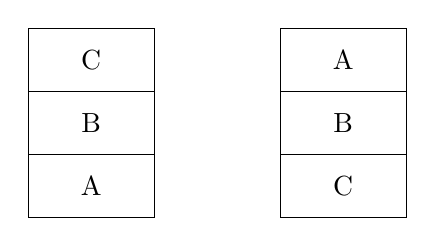
\begin{tikzpicture}[scale=0.8]
  % Initial configuration
  \draw (0,0) rectangle (2,1) node[midway] {A};
  \draw (0,1) rectangle (2,2) node[midway] {B};
  \draw (0,2) rectangle (2,3) node[midway] {C};

  % Goal configuration
  \draw (4,0) rectangle (6,1) node[midway] {C};
  \draw (4,1) rectangle (6,2) node[midway] {B};
  \draw (4,2) rectangle (6,3) node[midway] {A};
\end{tikzpicture}
\label{fig:intro-blocks}
\end{figure}

Planning tasks are solved by planners, which are software systems designed to find plans for given planning problems. Planners employ various algorithms and techniques to explore the search space of possible operators and states in order to find an optimal or satisfactory plan. Planners typically take as input a formal representation of the planning problem, including the initial state, goal condition, and a set of available operators. The formal representation of a planning task can be specified using planning languages such as PDDL (Planning Domain Definition Language).

\ppi{Continue...}

%Most planners use a best-first search algorithm such as greedy best-first search (GBFS)~\cite{doran-michie-rsl1966} to solve tasks. GBFS maintains states in a priority queue ordered by their cost-to-goal estimate, provided by the \emph{heuristic function}. GFBS finds a solution by first expanding states with the lowest cost-to-goal estimate. Several domain-independent heuristics efficiently compute the cost-to-goal estimate or heuristic value ($h$-value) of a state using the domain logic, i.e., specific information that enables reasoning about operators and other rules, such as mutexes that indicate impossible states. These heuristics are based mainly on techniques such as abstractions, delete relaxation, and landmarks~\cite{culberson1998pattern,haslum-geffner-aips2000,hoffmann-et-al-jair2004,Helmert.Domshlak/2009}. The heuristic function is the most important component of a planner since it guides the search.

%Using heuristic functions in conjunction with preferred operators can aid planners in reducing the number of expanded states during a search process~\cite{Richter.Helmert/2009}. By prioritizing the expansion of states generated by preferred operators, these planners benefit from additional guidance, often resulting in a higher success rate for solving tasks compared to modifying the heuristic function alone. The existing approaches for identifying preferred operators are limited to symbolic-based methods, and the current best is to use the preferred operators computed alongside the Fast-Forward (FF) heuristic~\cite{Hoffmann.Nebel/2001}, as implemented in the Fast Downward~\cite{Helmert/2006} planning system. Preferred operators are especially helpful in competitive settings to maximize the number of solved tasks: planners using preferred operators were the winners of the satisficing track of the \textit{International Planning Competition} (IPC) in the years 2004, 2008, 2011, and 2018~\cite{Helmert/2006,Richter.lama.etal/2011,Richter.lama.etal/2011,Seipp-fast.etal/2018}.


%
% - - - - - - - - - - - - - - - -- - - - - -
% background
% - - - - - - - - - - - - - - - -- - - - - -
% these are all things that exist already
% and that the reader needs to know before
%
\chapter{Background}

\section{Classical Planning}

\section{Greedy-Best First Search}

\section{Heuristic Functions}

\section{Preferred Operators}

\section{Residual Neural Networks}
\ppi{Needed?}

%
% - - - - - - - - - - - - - - - -- - - - - -
% sample generation
% - - - - - - - - - - - - - - - -- - - - - -
% now we talk about the stuff we're doing
%
\chapter{Sample Generation}

\section{Ideal Preferred Operators}

\section{Discovered Preferred Operators}

%
% - - - - - - - - - - - - - - - -- - - - - -
% experiments
% - - - - - - - - - - - - - - - -- - - - - -
% empiricism!
%
\chapter{Experiments}

\section{Configuration}

\chapter{Conclusion}

\bibliographystyle{abntex2-alf}
\bibliography{biblio}

\appendix

\chapter{Resumo expandido}

\noindent
\textbf{Resolução 02/2021 -- Redação de Teses e Dissertações em Inglês}
Dissertações de Mestrado e Teses de Doutorado do PPGC, bem como outros
trabalhos escritos tais como Proposta de Tese e PEP, poderão ser
redigidas em inglês desde que contenham um título e resumo expandido
redigidos em português. O resumo expandido deve conter no mínimo duas
páginas inteiras, deve aparecer como apêndice e deve conter as
principais contribuições e resultados do trabalho.


\end{document}
